\begin{figure}[tb] 
\centering
 \makebox[\textwidth]{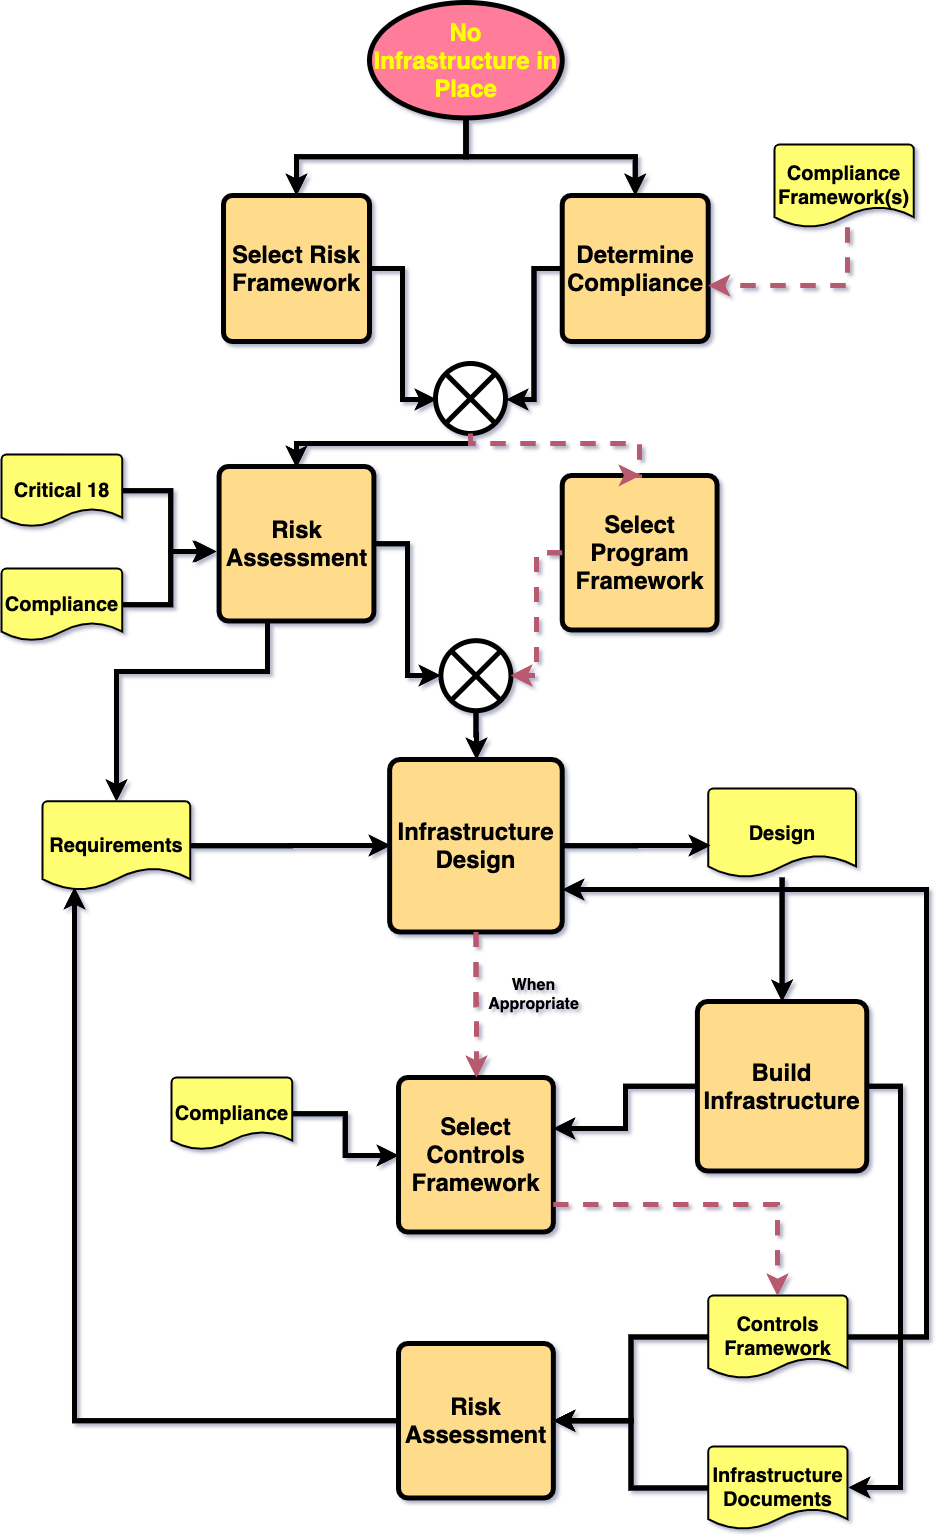
\includegraphics[height=\textheight,width=.9\paperwidth]{./figures/fig1.png}}
\caption{Frameworks Selection Process}
\label{fig:Fig1}
\end{figure}

\cleardoublepage

\begin{figure}[t!] 
\centering
 \makebox[\textwidth]{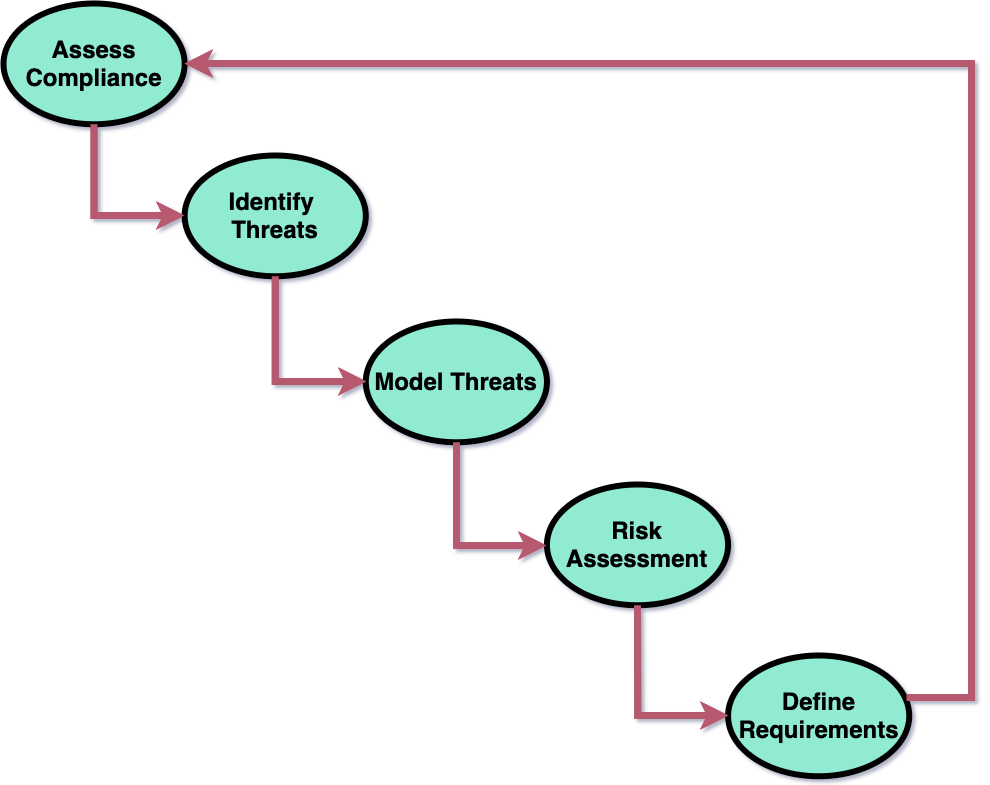
\includegraphics[scale=.45]{./figures/fig2.png}}
\caption{Requirements Definition Process}
\label{fig:Fig4}
\end{figure}

\begin{figure}[h!] 
\centering
 \makebox[\textwidth]{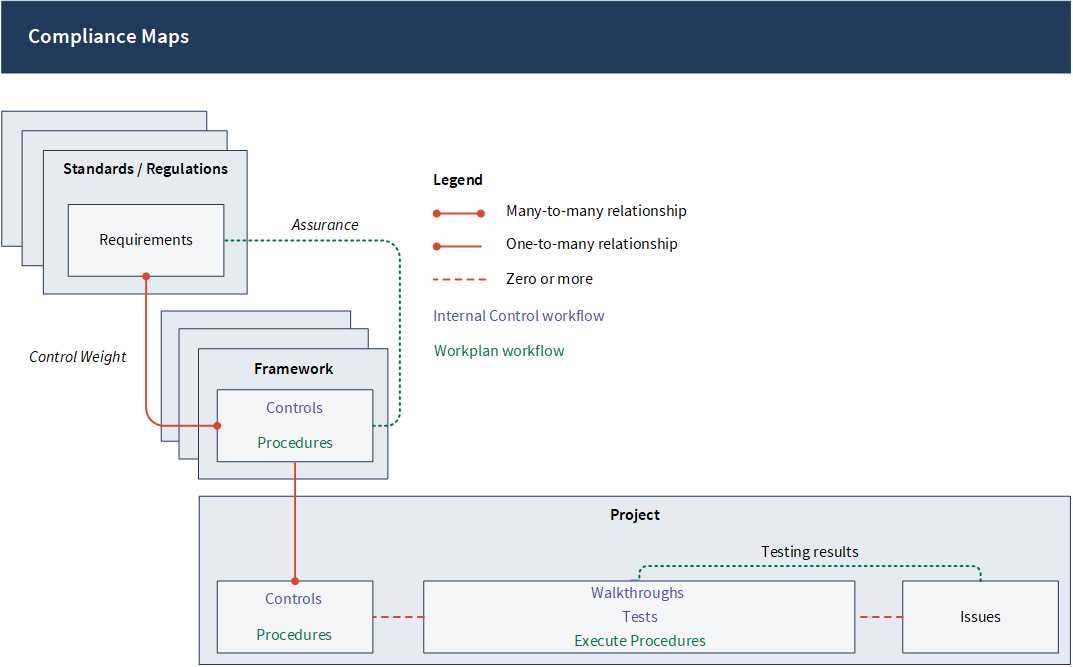
\includegraphics[scale=.45]{./figures/Compliance_Maps_ERD.png}}
\caption{Compliance Maps Entity Relationship Diagram (ERD)}
\label{fig:Fig5}
\end{figure}

\cleardoublepage

\begin{formal}
    
    \begin{quote} 
    \begin{minipage}{\linewidth}
    \stepcounter{footnote}
    \renewcommand\thempfootnote{\textcolor{orange}{\arabic{footnote}}}
    \setlength\parindent{15pt}
    
\par The processes for selecting a framework for a new or established business can differ based on the security program’s maturity.\ Figure \ref{fig:Fig1} shows the complete process.\ An organization starts its process at the appropriate point.\ In the real world, an organization might find itself anywhere on this model.\ The red dashed arrows are paths needed only initially or when business conditions radically change.\hfill
\vspace{10pt}
\par The first two steps can take place at the same time.\ They include selecting a risk framework and determining compliance.\ Determining compliance may also require adopting a compliance framework.\ For example, entities covered under the HIPAA need to understand the necessary standards before finalizing network and system requirements.\hfill
\vspace{10pt}   

\par The team needs a risk framework to guide the initial and future risk assessments.\ Each risk assessment includes compliance requirements.\hfill
\vspace{10pt} 

\par The initial risk assessment uses the compliance requirements and the modeling of probable threats to perform a risk assessment.\ This process is shown in Figure \ref{fig:Fig2}.\ If the organization has not yet selected a control framework, it should use the CIS 18 critical controls as a baseline until it adopts a more comprehensive framework.\footnote{\url{https://www.spiceworks.com/it-security/cyber-risk-management/articles/best-security-framework/}}

\begin{flushright}
--- Tom Olzak\\ 
Cybersecurity Researcher, Author \& Educator\\
July 29, 2021
\end{flushright}
\vspace{10pt}

    
    \end{minipage}
    \end{quote}

\end{formal}

Figure \ref{fig:Fig2} is featured in the video \href{https://www.youtube.com/watch?v=vKFtEt_i62o}{Select System Controls Based Upon Requirements}. I would also like to direct your attention to \href{https://www.auditscripts.com/resources/open_threat_taxonomy_v1.1a.pdf}{this document}. The taxonomy found therein is the final result of a research project conducted by Enclave Security. 

\cleardoublepage